% !TEX root = ../Article.tex
\chapter{Challenges and use cases}
In this chapter we will examine what challenges there are with regards to mobile devices and smart cards co-operating. The challenges must be viewed from a use case perspective where the benefits do not come from solving the challenges, but rather what we are able to achieve afterwards. For each challenge we will provide problem description, motivation, key concepts, possible solution and describe possible attack vectors.
\section{Binding card and phone}
\label{sec:bindingcardandphone}
\subsection{Problem Description}
%One of the key challenges when utilizing smart cards with mobile devices is establishing an initial trust relationship. How can the mobile device know that it communicates with a certified smart card (company/department issued) and how can the smart card know that it is interracting with a trusted user on a mobile device? To initialize this trust relationship we need to perform a handshake where we verify that all concerning parties can authenticate and authorize each other.
One of the key challenges when utilizing smart cards with mobile devices is establishing an initial trust relationship. How can the mobile device know that it communicates with a certified smart card (company/department issued) and how can the smart card know that it is interacting with a trusted user on a mobile device? The biggest problem of the binding process is that the smart card must trust the mobile device, as we have no way of knowing if we are binding to a compromised mobile device.  If the mobile device is not initially compromised and we are able to use the smart card as a bootstrap for trust, then the direct result is that we can use smart cards as a policy enforcement point (PEP) and secure key storage/generation. To initialize this trust relationship we need to perform a handshake where we verify that all concerning parties can authenticate and authorize each other.

\subsection{Goal}
By binding the smart card and phone together we wish to ensure that a smart card can only be paired with one mobile device and that we are in full control during the process. If we achieve this the direct consequences are:
\begin{itemize}
  \item The keys stored on the smart card cannot be retrieved or be used on a different mobile device.
  \item Our application on the mobile device cannot be used without the smart card that was paired with our mobile device.
  \item If the binding is successful we may be able to detect if the mobile device becomes compromised on a later point and react to it (delete keys on card, block communication, etc.).
\end{itemize}

This will mitigate vulnerabilities such as:
\begin{itemize}
  \item Lost or stolen device.
  \item Unsecure communication channels.
  \item Authentication challenges.
\end{itemize}

\subsection{Key concepts}
To authenticate the two parties, smart card and mobile device, we will need a third party which they both trust. We introduce a new party, the authority, which acts as a trusted third party. The authority issues the smart cards and employ the users. A direct consequence is that they both trust the authority, otherwise we have no starting point. Since they both trust the authority they can ask the authority to verify the other party as shown in figure \ref{fig:standardAuth}.

\begin{figure}[h!]
  \caption{Trust based on a third party.}
  \label{fig:standardAuth}
  \centering
    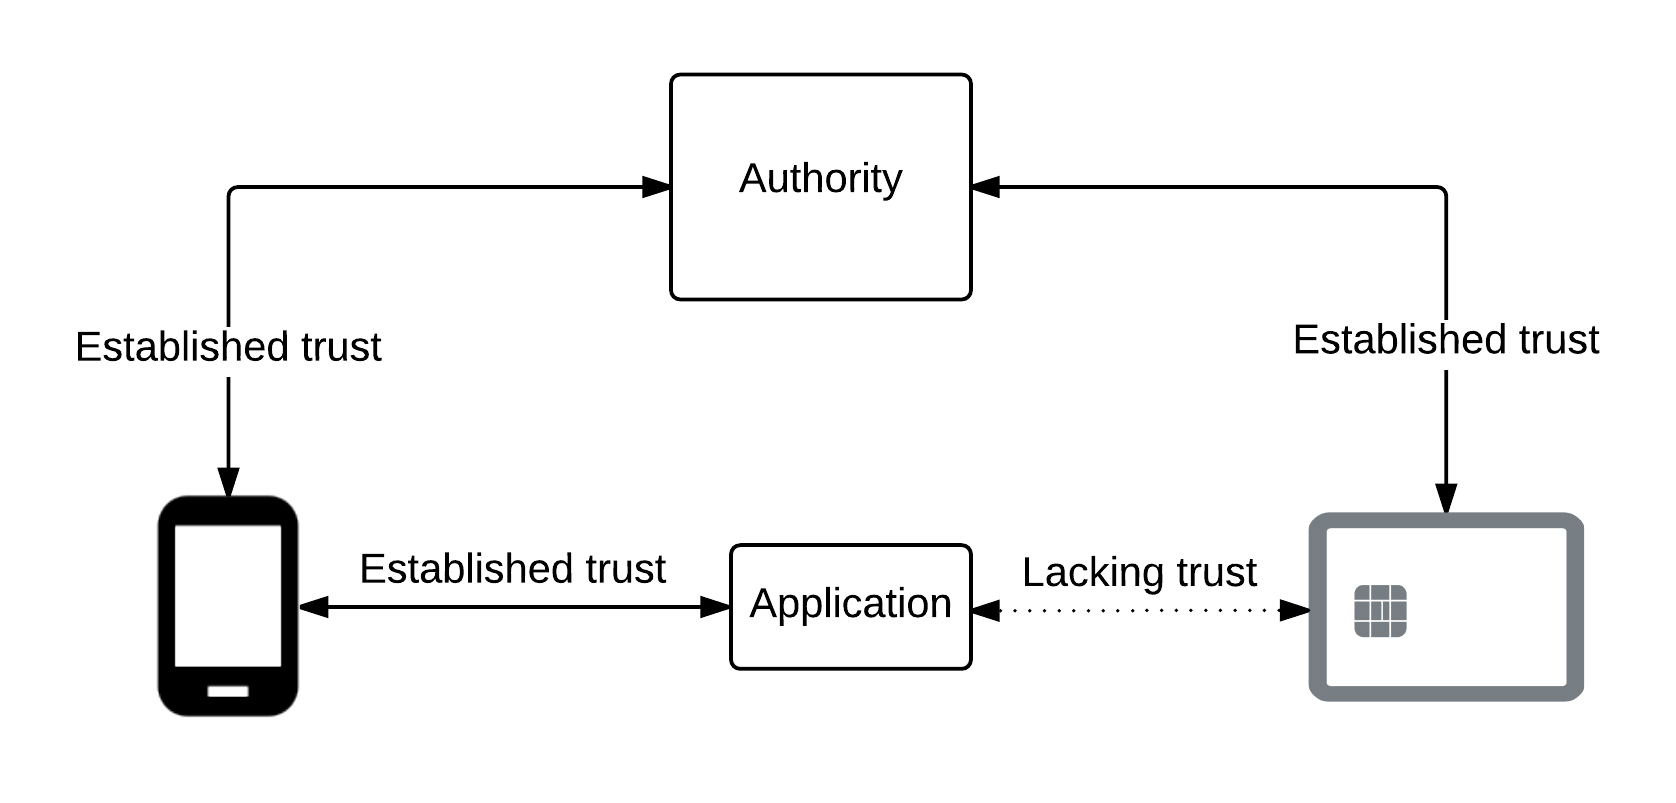
\includegraphics[width=0.95\textwidth]{images/standardAuth2.png}
\end{figure}

One thing that differentiates our challenge from traditional authentication challenges is that the smart card is not able to communicate directly with a trusted third party. All communication from our smart card to off card applications or third parties must go through a mobile device. A technical illustration of this relationship can be seen in figure \ref{fig:smu} where the authority is represented as a server. This drawback introduces a new problem which we have to consider. How do we know if the mobile device relays information between the server and smart card correctly in the authentication process?

\begin{figure}[h!]
  \caption{Server, mobile device and smart card communication flow.}
  \label{fig:smu}
  \centering
    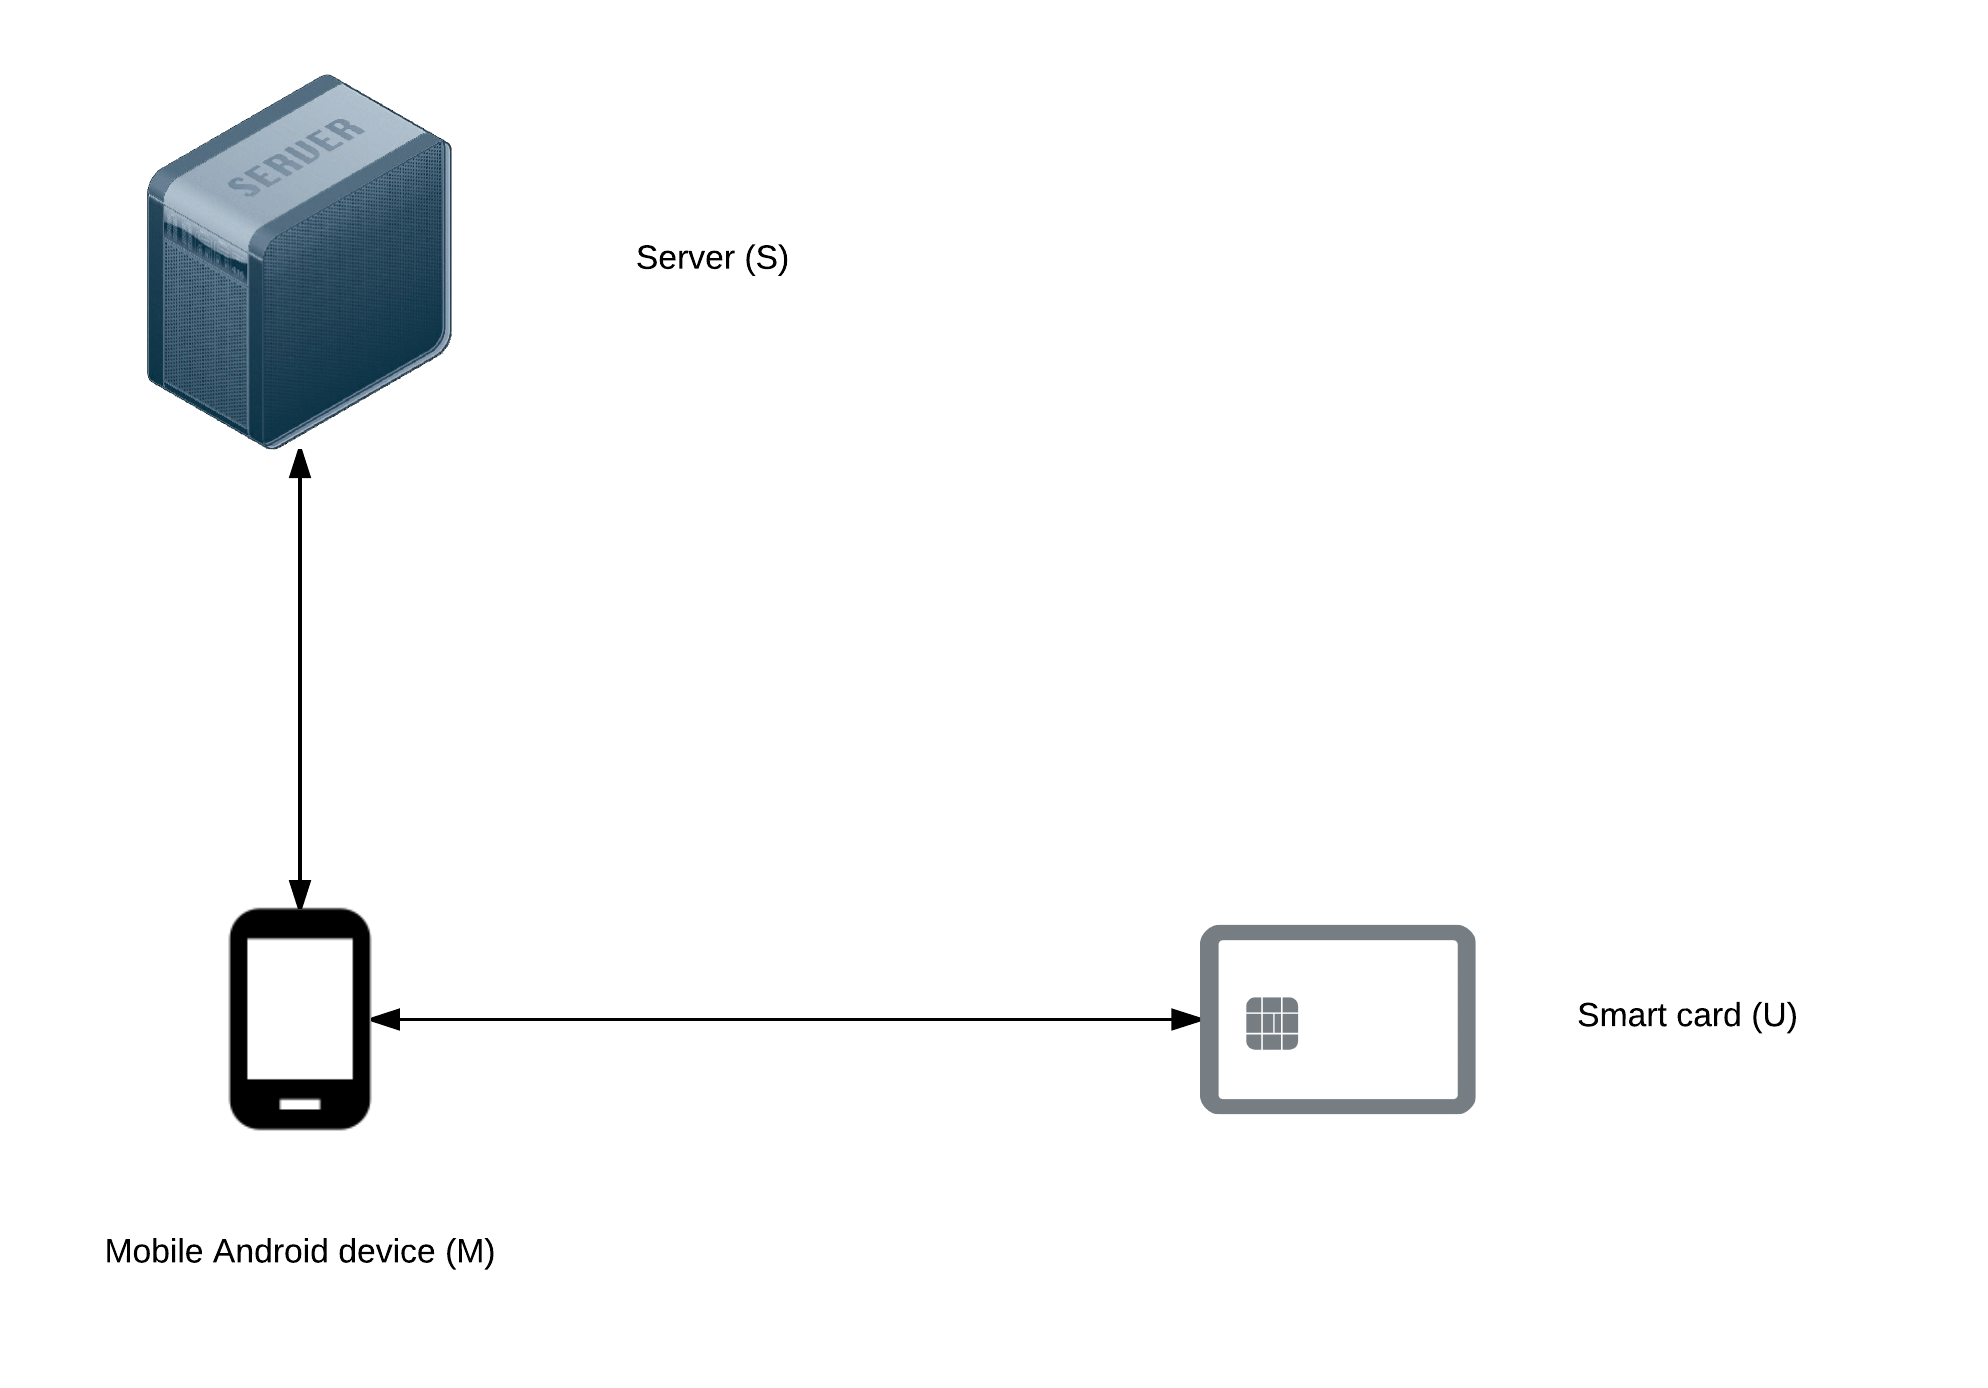
\includegraphics[width=0.95\textwidth]{images/SMU.png}
\end{figure}

To combat that all information flowing from the smart card has to go through the mobile device, we can utilize the fact that the authority we are trying to authenticate with is also the the smart card issuer. What this means is that we can pre-install the authority certificate and public key on the smart card as well as retrieve the public key of the smart card before handing the smart card to the user/employee. The result is that we have already exchanged the keys and certificates we need for authenticating the server and smart card before we introduce the mobile device.

The mobile device will also need to authenticate with the authority so that the smart card can trust the mobile device. In this process we will need to make some assumptions. The first problem is that we need to  ensure that the mobile device tries to communicate with the right server (authority). By hardcoding the server URL in the mobile device application and making sure that the user installs the right application on his device we can mitigate this threat. To make sure that the user installs the right application we need a secure distribution platform. By using Google Play as distribution platform, we can minimize the risk that the user will download a rogue application with the same name \cite{googlePlaySecureDist}. To further mitigate the risk of installing the wrong application the user can disable the ability to side-load applications and avoid using a rooted device.

The other attack vector on the mobile device and user is man-in-the-middle attacks. If we assume that the user was able to download the correct application we will need to secure the communication channel. To secure the channel we will need to use Transport Layer Security (TLS) \cite{rfc793} which also provides us with protection from replay attacks \cite[~Ch. 9.2.2]{TLS101}. The only downside by using TLS in our case is that we will need the server certificate to verify the server. Traditionally we will need to either pre-install certificates on the mobile device (makes ``bring your own device'' more difficult) or register with a certificate authority (depend on third party). In our case the server certificate is already on the smart card and we can install it on the mobile device. An added benefit of this is that if the mobile device is rogue and tries to connect to the wrong server; the data sent to the server will be encrypted by the smart card.

Further we will need the user to authenticate with the authority. We have two options in order to achieve this. First option is that users use a username and password combination directly with the authority, but considering the binding is normally a one time case a more simplified process may be to hand out a one time code along with the smart card. One could also look into distributing one time codes through e-mail or a text message (SMS).

The second option is that the user inputs a pin code to the smart card and if the pin code is correct the smart card can verify that the user is the user he claims to be. This option requires very little overhead and saves a lot of resources in that regard.

We have described how the parties can authenticate each other, but we will need to describe this as a unified process (refer to section \ref{sec:proposedSolution}) and identify attack vectors and weaknesses (refer to section \ref{sec:attackVectors}).

\subsection{Proposed solution}
\label{sec:proposedSolution}

\paragraph{Pre-conditions}\mbox{}\\
The authority issues the smart cards and administrates the server. During the setup of the smart card the public key and certificate of the server must be installed on the smart card. The public key of the smart card must also be extracted and stored on the server. This creates a base for all future processes.

\paragraph{Verification package}\mbox{}\\
A verification package is a package containing all the information a third party server needs to authenticate the smart card and mobile device. First the mobile device public key and the generated AES key is signed by the smart card. Then we encrypt the package with the public key of the third party server. Figure \ref{fig:h0} visualizes this structure.

\newpage

\begin{figure}[h!]
  \caption{Verification package structure.}
  \label{fig:h0}
  \centering
    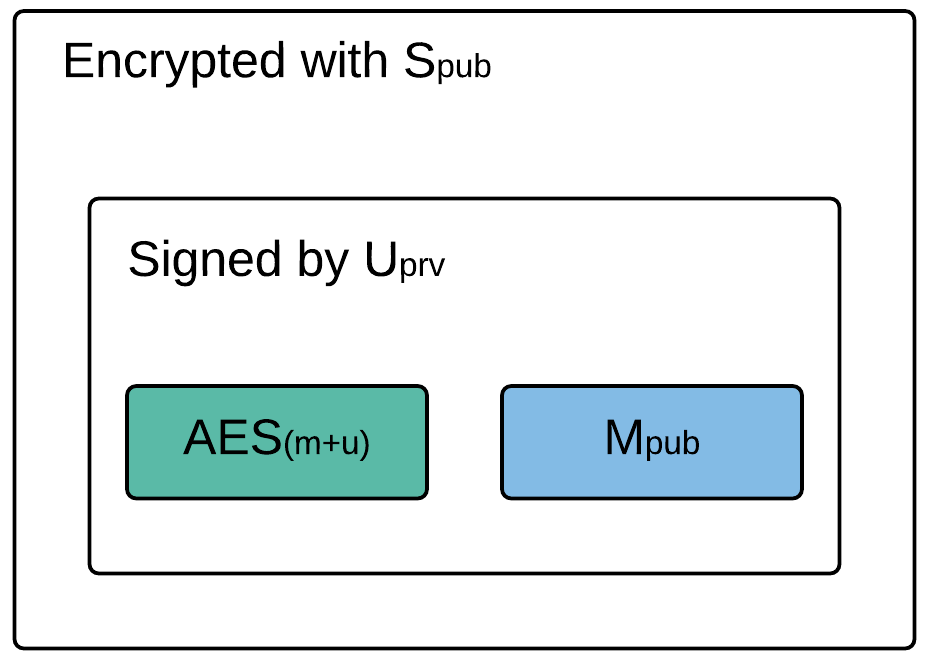
\includegraphics[width=0.95\textwidth]{images/H0.png}
\end{figure}

We propose the following protocol for binding mobile devices and smart cards:

\paragraph{Abbreviations}\mbox{}\\
U - Users smart card \\
M - Mobile device \\
S - Server, representation of authority \\
H\textsubscript{0} - Verification package \\
\{Entity\}\textsubscript{pub} - Public key of an entity (U, M, S)\\
\{Entity\}\textsubscript{prv} - Private key of an entity (U, M, S)\\
\{AES\}\textsubscript{Entity+Entity} - AES key of two entities (U, M, S)\\


\begin{enumerate}
  \item Install Android application on mobile device (M) and insert smart card (U).
  \item M generates RSA key-pair and stores it.
  \item M sends M\textsubscript{pub} to U and requests verification package (H\textsubscript{0}) from (U).
  \item U asks for a PIN code.
  \item M provides PIN code.
  \item U generates H\textsubscript{0} (refer to figure \ref{fig:h0}) and sends it to M.
  \item M connects to the server (S) and sends (H\textsubscript{0}) to S.
  \item S decrypts (H\textsubscript{0}) using S\textsubscript{prv} and verifies the signature of U.
  \item S saves AES\textsubscript{(M+U)} for safekeeping, signs M\textsubscript{pub} and sends the signed  M\textsubscript{pub} to M.
  \item M forwards the signed M\textsubscript{pub} to U.
  \item U verifies that M\textsubscript{pub} was signed by S and if successful U sends U\textsubscript{pub} to M.
\end{enumerate}

\newpage
\begin{figure}[h!]
  \caption{Sequence diagram for binding mobile device with smart card.}
  \label{fig:sqd}
  \centering
    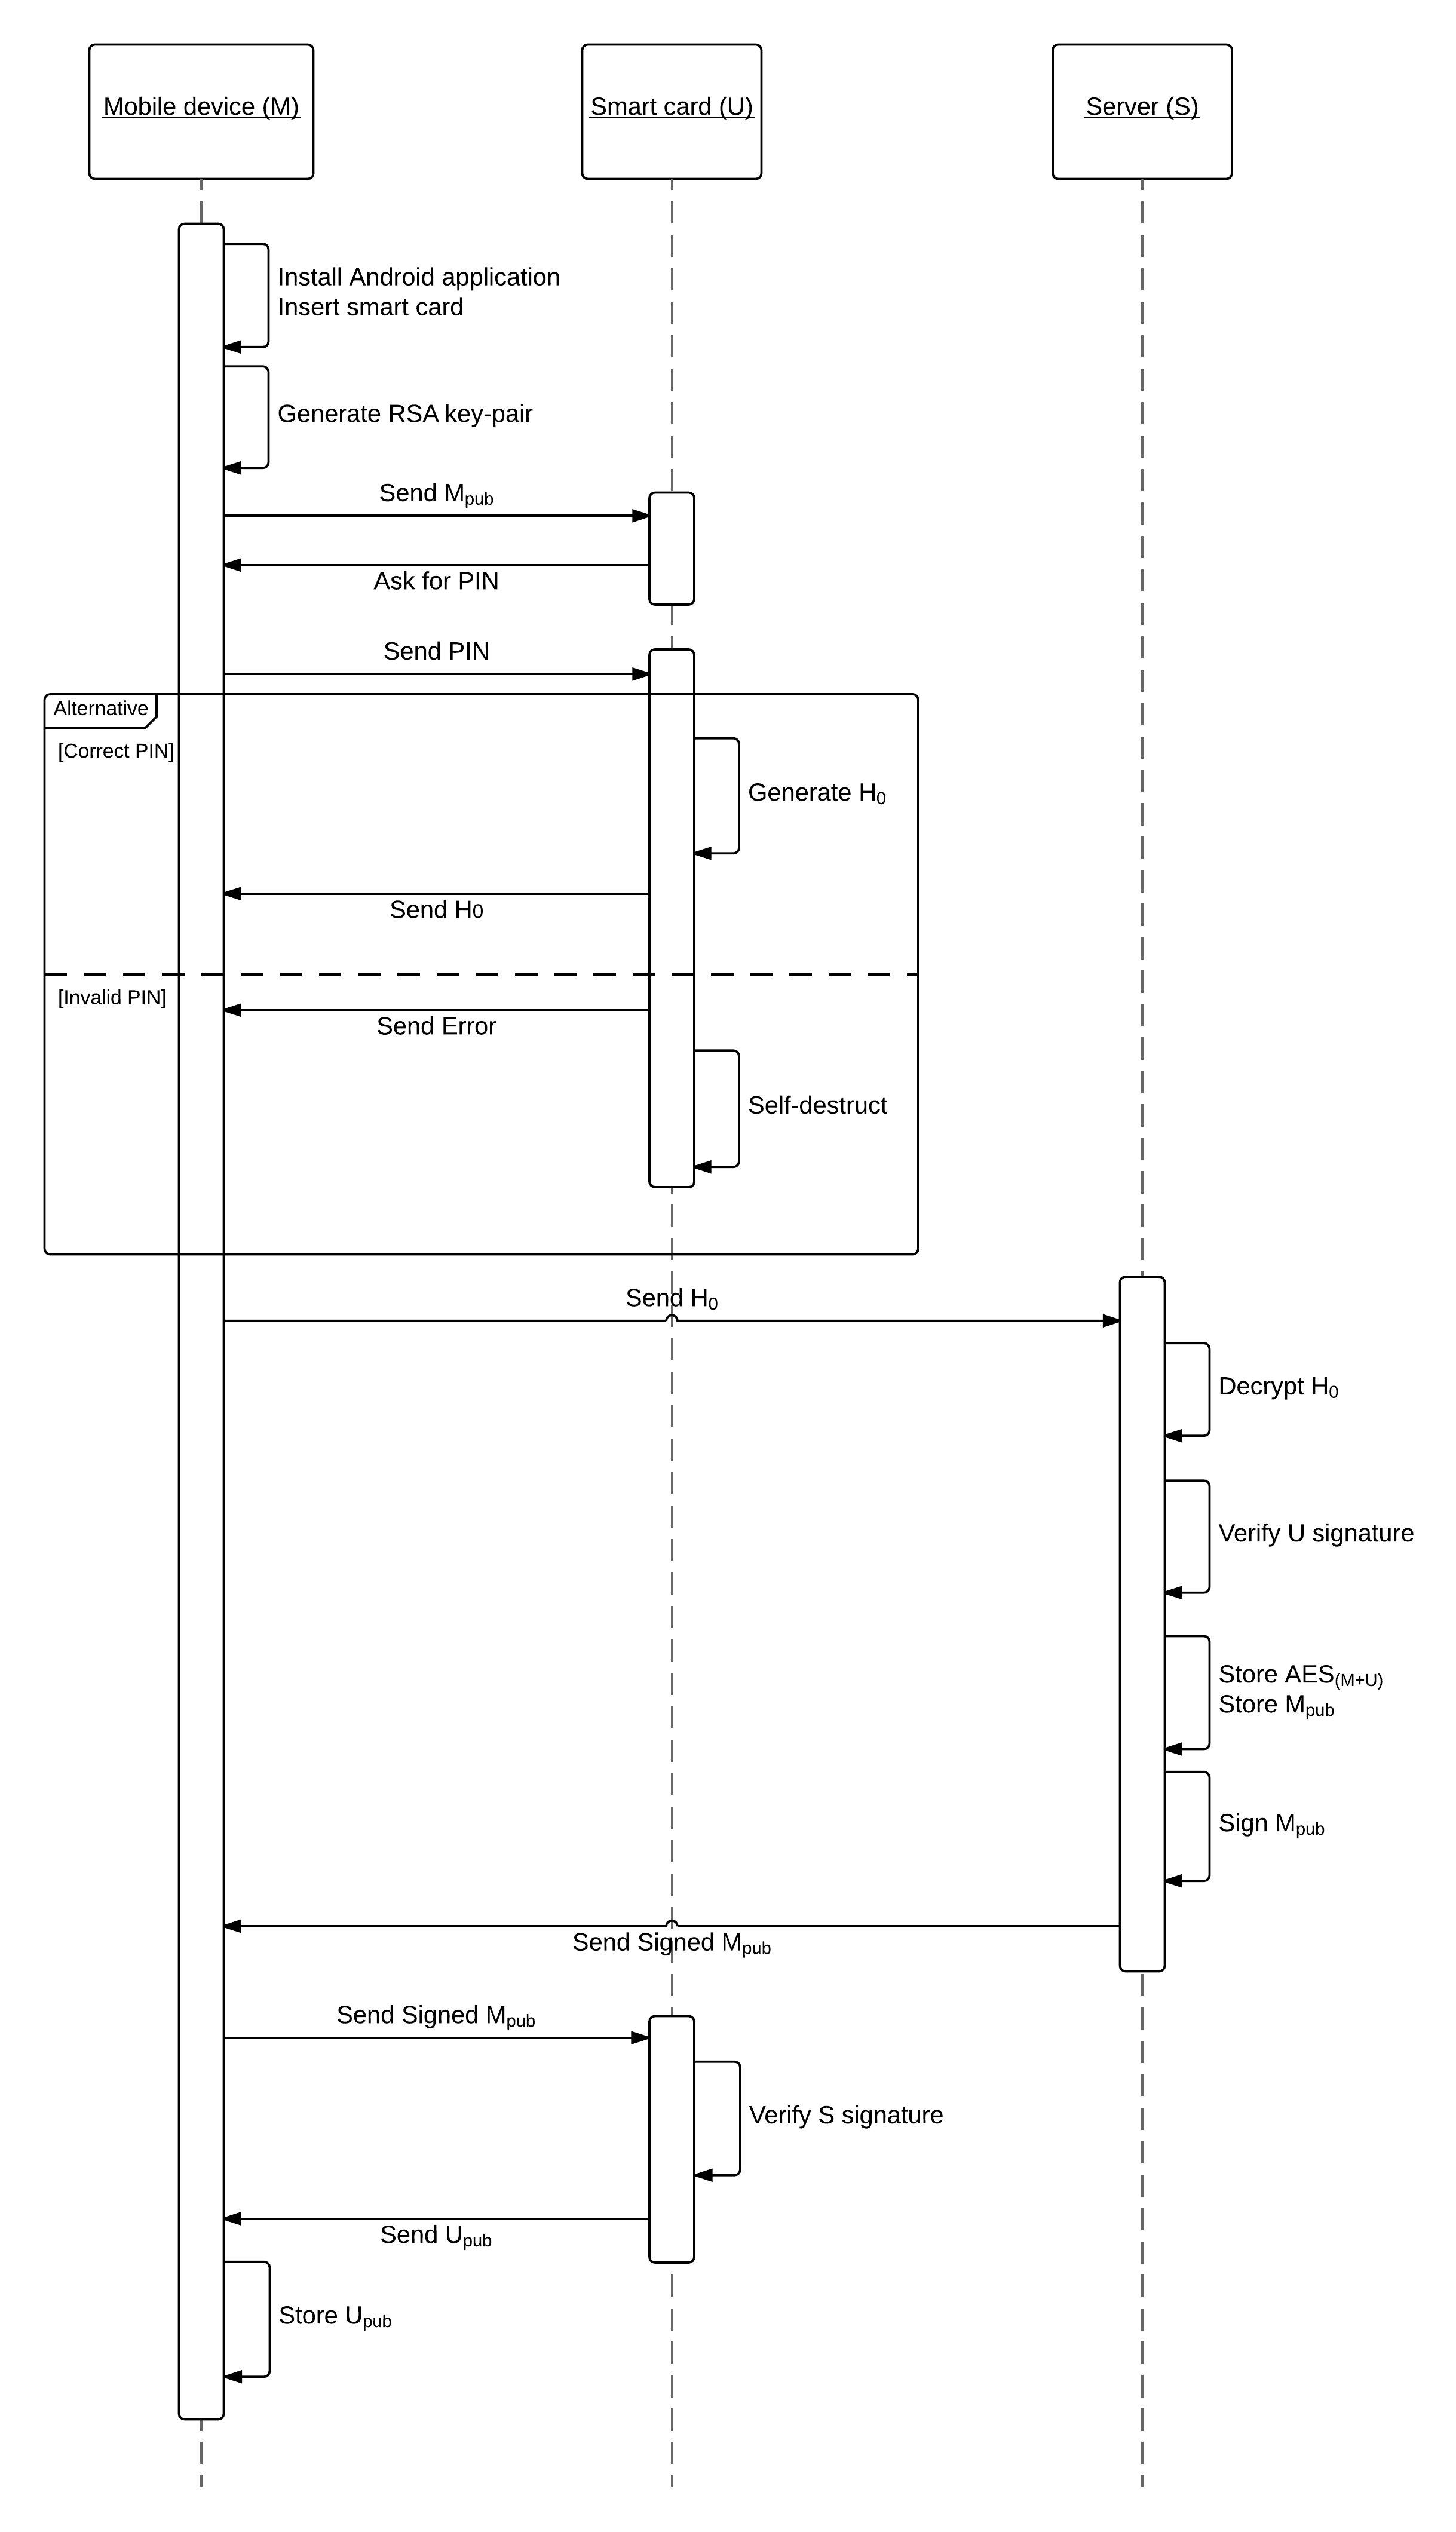
\includegraphics[height=0.93\textheight]{images/SQD_handshake.png}
\end{figure}
\newpage
The end result of the transactions is that the smart card and mobile device have shared their public keys through the trusted third party and can thus communicate securely. The server will also have a record of the transactions and the parties. If we chose to do so we can also save a backup of the first symmetric key on the server.

Potentially we could add more steps to the process to further heighten the security. In step 7 we could add that a user may need to answer a challenge such as provide a one time password (OTP). This would add more overhead and require more resources administrating.

A direct consequence of a successful binding is that the smart card is now locked to the mobile device. Inserting the smart card into a different device will simply not work due to the fact that the smart card has the public key of the original device and they have already agreed upon a symmetric key. To further enhance this trait we can once in a while challenge the mobile device which requires the private key of the original bound device to solve (e.g. challenge is encrypted with M\textsubscript{pub}).

\subsection{Architecture evaluation}
In this section we will justify and evaluate the parts of the solution that have security implications.

\paragraph{M generates RSA key-pair and stores it.}\mbox{}\\
For the smart card to bind itself to a mobile device we need a unique identifier or key that no other device is able to replicate or spoof. An RSA key-pair provides this functionality as the mobile can use the private key to sign data and the smart card can encrypt data with the mobile device public key. Unless another mobile device is able to extract the private key we are in the clear security wise. More on this and other solutions in section \ref{sec:mobileDeviceKeys}.

\paragraph{U asks for PIN code.}\mbox{}\\
We chose to add a PIN code step to the binding process to add another layer of security. The PIN code ensures that a person is verified by the employer to perform the binding process. Using PIN codes is not a guaranteed measure against someone unauthorized trying to carry out the binding process. The important steps to make sure the PIN code process is secure are:
\begin{itemize}
  \item The binding process should be carried out as soon as possible after obtaining the PIN code to avoid someone leaking or losing the PIN code.
  \item Add a limited number of tries for inputting the PIN code on the smart code to mitigate brute-force attacks.
  \item In connection to the previous point; the PIN code length should correspond to the number of tries.
\end{itemize}

\paragraph{U generates the verification package.}\mbox{}\\
The smart card is a secure environment and should be in charge of generating the verification package. We include the AES key for safekeeping on the server incase the user lose the smart card. We sign the package using the private key of the smart card and the server can verify that it is a legit smart card since the server has the public key. This step is necessary as anyone would be able to send a verification package to the server as the server public key is public. Lastly the smart card encrypts the verification package using the server's public key. The end product, the verification package, is secure in the sense that only the server can read the data and the server can authenticate the sender using the signature.

\paragraph{M connects to the server (S) and sends the verification package to S.}\mbox{}\\
The verification package is encrypted with the server's public key. The direct result is that even if the package is lost or leaked no third party would be able to read the content. We will use TLS for the connection regardless as it may be necessary to add additional functionality such as username-password login to verify the user. TLS will also serve as a counter to replay-attacks and man-in-the-middle attacks.

\paragraph{The server signs the public key of M.}\mbox{}\\
The server signs the public key of the mobile device. This is done because of the need to confirm that the verification package was indeed sent to the server. By letting the server sign it we ensure that the public key that is sent back to the smart card is in fact the public key that was in the verification package.

\paragraph{U verifies that M\textsubscript{pub} was signed by S and if successful U sends U\textsubscript{pub} to M.}\mbox{}\\
Even though public keys usually are publicly known we choose to keep the public key of the smart card semi-public or on a ``need to know basis''. Using this technique F not inherently make the solution secure, but it does add another hurdle a potential attack will need to overcome. In theory, the more steps an attacker will need to do; the higher the chance for detecting him. By rotating the keys the effectiveness of this measure increases substantially.


\subsection{Cryptography evaluation}
This solution relies heavily on correct use of protocols such as TLS (communication), cryptography such as RSA and AES, and correct key generation.

One of the most common public-key cryptosystems (refer to section \ref{sec:publicKeyCrypto}) is RSA, which is widely used for secure communication. RSA builds on the principle of factorization of the product of two prime numbers, or rather the difficulty of factorize the product. It is not impossible to factorize the product of two prime numbers and there was a challenge by the RSA Laboratories where one could win prizes for factorized RSA-keys \cite{rsaChallenge}, but the most complex RSA that were cracked was 768-bit. Proving that RSA is secure is out of the time scope for this thesis. Other source conclude that with long enough keys and correct protocol implementation, the math behind RSA can be considered secure \cite[~p. 194]{cryptoMath}. Information on the inner workings of RSA can be found in the book ``Understanding Cryptography'' by Christof Paar and Jan Pelzl, chapter 7 ``The RSA Cryptosystem'' \cite{cryptoMath}.

We are not directly utilizing the symmetric-key cryptography system AES, but it is an important aspect of the solution none the less. AES does not rely on number factorization, but rather substitution and permutation using a key. It can be seen as hashing data and being able to reverse the hashing using the same key. There are currently no known analytic attacks against AES which are less complex than brute-force attacks and we can thus conclude that using long keys are to be considered secure \cite[~p. 116-117]{cryptoMath}.

In the solution we mitigate man-in-the-middle attacks using TLS for secure communication. TLS can utilize both RSA and AES and if we use strong keys we deem it secure (assuming TLS 1.2) from a mathematical perspective. If TLS is implemented correctly and does not allow for common attacks (Heartbleed, DROWN \cite{drown}, , etc.) it is classified as ``probably secure'' or ``secure until proven otherwise''.
%TODO


\subsection{Potential attack vectors}
\label{sec:attackVectors}
%This solution relies heavily on correct use of protocols such as TLS (communication) and correct key generation. We assume that all cryptographic functions we use are used correctly and all keys are of such lenghts that they are cryptographically strong. Now that we have established that requirement we can look at the different attack vectors.

\paragraph{Rogue technical party}\mbox{}\\
The three technical parties involved are the server, the mobile device and the smart card. As discussed previously ``the authority'' issues the smart cards and administrates the server. Since the public keys and certificates are exchanged before the smart card is distributed the server is able to detect if there are a rogue/fake smart card trying to bind to a mobile device. If the mobile device tries to connect to the wrong server (man-in-the-middle attack, wrong URL, etc.) and the server tries to pose as a legit server, it will not be able to complete the binding process due to needing the matching private key for the public server key on the smart card.

Thus the only attack vector on technical parties is where the mobile device is rogue. By rogue in the context of the mobile device we mean compromised as in rooted or malware/spyware. In our solution we have no way of knowing if the user is binding a rogue mobile device. The end result is that we have securely bound the mobile device and smart card, but the mobile device cannot be trusted.

To combat this we need to do two things. First and foremost we need to educate the user on mobile security and how they should not install applications from untrusted sources etc. Secondly we can run tests on the mobile device to try and detect if the mobile device is rooted or has malware/spyware. This can prove to be hard as it is very difficult, if not impossible, to detect malware/spyware which operate with root access. Google has been working on a security framework, SafetyNet, which goal is to detect if a device has been tampered with or is infected \cite{googleSafetynet}. In order to decide if this is sufficient we would have to do more research on SafetyNet specifically.

\paragraph{Rogue user or administrator}\mbox{}\\
Potentially we can have a rogue user which deliberately installs malware/spyware on their mobile device to compromise our system. We will disregard this case as if we have a rogue user we have bigger problems than a compromised mobile device. It is also important to note that any information the mobile device receives the user is also likely to know regardless, and can thus release this information independently of the mobile device.

The bigger problem would be a rogue administrator. The administrator would have access to the initial setup of the smart cards and may extract the private key of the server. Even though this has more impact than a rogue user we are very limited on what we can to do protect against it. We can make it near impossible to extract private keys, logging and require more than one administrator, but it will still be possible to cause harm. Although the same principle applies here: if you have a rogue administrator you have bigger problems than smart card binding.


\subsection{Additions}
In step 9 and 10 of the proposed solution we can add a payload to the signed M\textsubscript{pub}. One of the uses for this payload may be to send information on how the smart card should handle communication, key generation, encryption \& decryption as well as administration. More on this in section \ref{sec:policies}.


\section{Mobile device keys}
\label{sec:mobileDeviceKeys}


\subsection{Problem statement}
Even though one of the features of the smart card is to store and manage keys we are still dependent on the mobile device being able to store at least one set of keys. This is directly tied to the binding process of the mobile device and the smart card which were discussed in section \ref{sec:bindingcardandphone}. The problem lies in the fact that how do we ensure that the key pair are generated and stored securely? By solving this problem we are able to perform the binding process of the mobile device and smart card. We can also envision that there might emerge other use cases at later stages which require keys on the mobile device.

\subsection{Goal}
Our primary goals for mobile device keys are:

\begin{itemize}
  \item Generate keys on mobile device or receive externally generated keys.
  \item Store keys securely on the mobile device.
\end{itemize}

\subsection{Key concepts}

\paragraph{Android Keystore system}\mbox{}\\
The Android Keystore system is a system that lets users and developers store and access cryptographic keys and certificates on the mobile device. The main goal of the system is to protect the keys against unauthorized use and extraction. This is done by defining which applications that should have access to the keys stored. E.g. application A generates and stores a key and defines that the key is available to application A and B. If application C tries to access the key the Android Keystore system blocks the action.

The applications do not have direct access to the keys. If an application wants to perform a cryptographic operation it feeds the data to the operating system which performs the cryptographic operation. If an application is compromised an attacker gains access to the keys via the application, but the attacker is not able to extract the keys as the keys are never present in the application.

In early iterations the keys were stored in a software-protected file meaning that only the Android Keystore had access to the data. This system had a flaw in which any users or applications with root access could access the Keystore file. The solution to this is using secure hardware such as ``Secure Element'' (more or less a smart card) and ``Trusted Execution Environment (TTE)'' \cite{TEE}. If hardware-backed storage is enabled (as seen in figure \ref{fig:hardwareBacked}), it is not possible to extract keys even if the operating system is compromised.

\begin{figure}[h!]
  \caption{Screenshot of Android settings showing hardware-backed storage ``enabled''.}
  \label{fig:hardwareBacked}
  \centering
    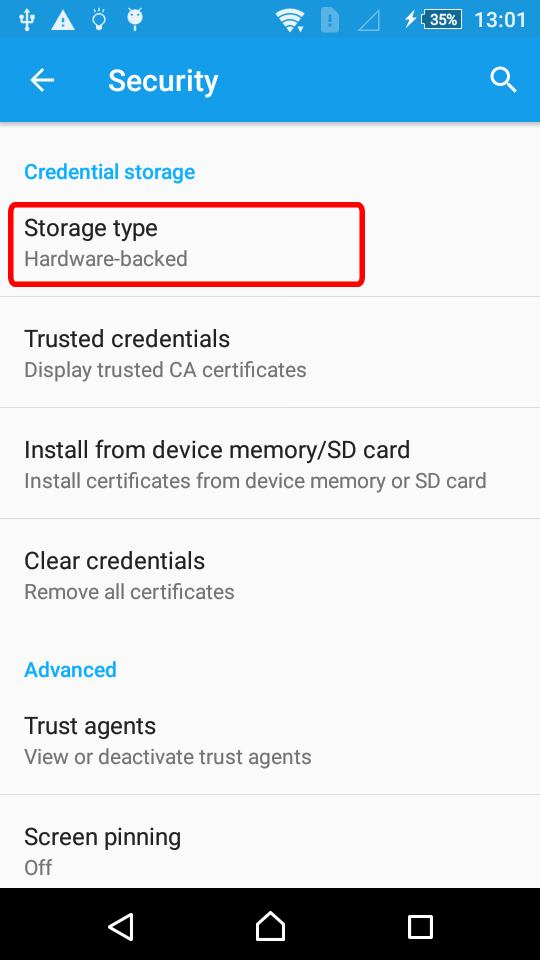
\includegraphics[width=0.45\textwidth]{images/hardwareBacked.png}
\end{figure}

An application can check if the mobile device uses secure hardware for key storage using the Android class \texttt{KeyInfo}. The \texttt{KeyInfo} class contains all available information about a key and a single call to the method \texttt{\allowbreak isInsideSecureHardware()} will determine the storage status. Listing \ref{lst:KeyInfo} provides a sample implementation of this functionality. \texttt{KeyInfo} was added in API 23 and requires Android version 6.0 or newer.

\newpage
\begin{lstlisting}[caption=Obtaining storage status of keys using KeyInfo., label=lst:KeyInfo,escapechar=å]
public boolean checkStatus(PrivateKey key){
    KeyFactory factory = KeyFactory.getInstance(
        key.getAlgorithm(), "AndroidKeyStore");
    KeyInfo keyInfo;
    try {
         keyInfo = factory.getKeySpec(key, KeyInfo.class);
        å\colorbox{highlight}{return keyInfo.isInsideSecureHardware();}å
    } catch (InvalidKeySpecException e) {
        // Not an Android KeyStore key.
    }
    return false;
}
\end{lstlisting}

\subsection{Generate keys on mobile device}
To generate keys on the mobile device an application must initialize the classes \texttt{KeyGenerator} or \texttt{KeyPairGenerator}. \texttt{KeyGenerator} is used for generating symmetric secret keys and the most notable supported algorithms are AES(up to 256-bit), HmacSHA256 and HmacSHA512. As the name suggest \texttt{KeyPairGenerator} is used for generating key-pairs. Pre API level 23 it was possible to generate DSA key-pairs, but the support was removed in favour for more secure algorithms. The two main supported algorithms are RSA (up to 4096-bit) and Elliptic Curve algorithms (P-224, P-256, p-384 and P-521).

Generating long keys may put some strain on the mobile device and should either be done in an asynchronous thread or during a setup process on first time launch of the application. However this should not be a deciding factor of whether or not the mobile device should generate its own keys as it is a one time process. Listing \ref{lst:keygenAndroid} shows how an application can use \texttt{KeyPairGenerator} to generate a 4096-bit RSA key-pair.

\begin{lstlisting}[caption=Generating RSA key-pair on Android device using KeyPairGenerator, label=lst:keygenAndroid,escapechar=å]
public KeyPair generateKeyPair(){
    KeyPairGenerator kpg = KeyPairGenerator.getInstance("RSA");
    kpg.initialize(4096);
    return kpg.generateKeyPair();
}
\end{lstlisting}

\subsection{Generate keys on server //p12-fil etc.}
\label{sec:generateKeysOnServer}
The Android Keystore system accepts \textit{PKCS\#12} archive files which it then stores on the mobile device. The PKCS\#12 file can contain certificates, keys and key pairs \cite{pkcs12}. After the archive file is manually installed on the device, applications that are authorized are free to use the keys via the Android Keystore system. The consequence of this is that we do not have to rely on the mobile device to generate the secure keys.

The most interesting characteristic of this solution is that a company or a similar entity can have a dedicated server generating these archive files. The server is able to run more security software than a mobile device and can be treated as a secure environment for key generation.

The PKCS\#12 archive file can be protected by a password and should definitely be protected by one to be even considered secure. This does add more overhead to the process of distributing the PKCS\#12 files.

The biggest obstacle when using server generated keys is distribution. You do not want to hand the PKCS\#12 file to the user on a USB stick along with a password on a notepad as you cannot be sure that the USB is destroyed or wiped properly along with the password. The solution to this is hosting the PKCS\#12 file on a website. The only way to access the PKCS\#12 file is through a portal which requires two-factor authentication (or similar) which limits user to only access the PKCS\#12 file they are supposed to reach. The file is then downloaded onto the mobile device and the users can install the file from their device memory (see figure \ref{fig:hardwareBacked}).

This solution does not remove the need for the users to know the password for the PKCS\#12 file and the file will still reside in the device memory. The only solution to this is to have strict security policies where the memory is wiped afterwards as well as removing the accessibility of the PKCS\#12 file on the server (from a users perspective).

\subsection{Evaluation and comparison}
In the problem statement we pointed out the binding process being dependent on the security of the keys generated and stored on the mobile device. We know that we are able to store the keys securely on the mobile device as long as hardware-backed storage is enabled and is being used. It is also possible to check if a key is stored on hardware in an Android application. In other words we have a solution to the storage issue: Use a mobile device which supports hardware-backed storage and validate it in the Android application using \texttt{KeyInfo}. The white paper ``Analysis of Secure Key Storage Solutions on Android'' by Tim Cooijmans, Joeri de Ruiter and Erik Poll discusses hardware-backed storage further \cite{KeyStorage}.

Security-wise the key generation on the mobile device and on a server is very similar. If the key generation on the mobile device is done correctly with properly generated secure initialization vectors the process is considered secure. The only realistic attack vector on key generation is that the mobile device is running a custom operating system which has it's own implementation of how key generation is done. To combat this scenario it may be necessary to use Google's security framework, SafetyNet, as mentioned in section \ref{sec:attackVectors} when we discussed attack vectors on the binding process.

The biggest benefit of generating the mobile device keys on a remote and secure server is that we can strengthen the insecure elements of the binding process. In the proposed solution of the binding process (section \ref{sec:proposedSolution}) we have to trust that the mobile device is a device that are supposed to perform the binding process. For example if an attacker is able to get his hands on a smart card before it is bound to a mobile device, he may try to start the binding process with his own device. We counteract this with requiring PIN code and the possibility of adding user authentication with the server. If the mobile device keys are pre-generated by a server and installed by an administrator on the mobile device we can use these keys to verify that the device is authenticated (as other devices does not have the keys). A consequence to this is that we may be able to simplify some of the steps in the binding process as we can trust the mobile device.

The drawbacks of pre-generating the keys apart from more overhead are the distribution process which in turn introduces new attack vectors. In section \ref{sec:generateKeysOnServer} we discussed how we could use a web server to distribute the keys. What is also worth mentioning is that this solution requires a web server to be maintained and protected. Such a system also places a lot of trust in the user's hands as he is responsible for deleting the PKCS\#12 file as well as not disclosing the password.

An other distribution solution is to have a trusted administrator install the keys on the mobile device. For some organizations this could be cumbersome as now all users will need to visit the ``headquarters''. This is a direct hindrance to the ``Bring your own device''-idea and can potentially introduce extra costs when it comes to human resourcing. Another key point to keep in mind is what should the protocol be if the organization wishes to update all keys? This would put a lot of stress on the distribution department.

There is no definitive ``best solution'' to the key generation problem. It all boils down to the question: ``Can you afford the infrastructure needed for server generated keys?'' If the answer to that question is yes then there is a lot to gain by using server generated keys as we have discussed above. Opting for the cheaper solution, generate keys on mobile device, does not equal an non-secure solution, but we do sacrifice some control of the process.


\section{Security policy enforcement}
\label{sec:policies}

\subsection{Definition}
A security policy defines what measures a system needs to follow in order for the system, organization, group, etc. to be secure. Security policies are not necessarily a technological restriction/rule and can exist as a socially enforced rule. Examples of security policies are:
\begin{itemize}
  \item All employees needs to have a background check.
  \item All company doors will be locked after 4 pm.
  \item Password must be changed once a month.
  \item Sensitive data must be encrypted with AES-256.
\end{itemize}

\subsection{Problem description}
Enforcing security policies via a mobile device is not a new concept and there exists multiple third party solutions for enforcing them. One example is Microsoft Exchange ActiveSync which enforces policies such as minimum password length, disable camera and application blocking \cite{exchangePolicies, msExchangeCookBook}. ActiveSync utilizes the fact that a user must connect through Microsoft Exchange Server in order to access company resources and verifies if the mobile device has enforced the policies through the established connection \cite{exchangePoliciesTech}.

The problem in these types of solutions lies in the fact that you cannot trust the mobile device to actually enforce the policies. How does the server know if the mobile device is telling the truth about policy enforcement? What if the mobile device says it requires the user to enter a password, but does not do it?

\subsection{Goals}
By using smart cards in the context of policy enforcement we wish to achieve the following:
\begin{itemize}
  \item Policies are enforced.
  \item Not possible to spoof policy enforcement by the mobile device.
  \item Policies cannot be tampered with.
\end{itemize}
Optionally we want to achieve the following:
\begin{itemize}
  \item Policies can be updated.
\end{itemize}

\subsection{Shift responsibility to a trusted party}
One way of making sure that policies are enforced is to give the responsibility of the action to a trusted party. Imagine that company A have a policy which requires their employees to update their password on their personal computers once a month. If the user profiles only exists locally on the computers, company A has no way of checking if the users update their passwords and run the risk of the users saying they have updated the password without doing so. To combat this the user profiles are moved to company A's server and the personal computers now do a lookup for the user profiles on the server. In this case, A has control over the user profiles and can check if the passwords are updated.

The limiting factor to a solution like this is that the trusted party might not be able to perform the job. A trusted server might not be able to enforce locking doors after 4pm just as a smart card is not able to perform all jobs we want it to do. A big part of the job is to identify which part of a security policy action we can move to the smart card to enforce the security policy.

\subsection{Proposed solution}
\label{sec:policySolution}

\paragraph{Relevant policies for a smart card}\mbox{}\\
The smart card is limited in what kind of policies it is able to enforce. It cannot enforce policies regarding forcing the mobile device into doing things only the mobile device controls. The smart card can provide vital data needed for performing an action, but it is up to the mobile device to actually perform the action. This effectively rules out policies such as, ``The mobile device must encrypt all files stored locally.'', since we can only provide the keys to do so, but the mobile device has to perform the action. We have to assume that the mobile device, more specifically the running application, wants to perform the action.

The core abilities of a smart card are: generate keys, store keys, encrypt and decrypt small amounts of data, sign data and store variables. We can make the application rely on the keys generated and stored in the smart card and as a result we have full control over the keys. The smart card can as a result enforce policies such as key rotation, key size and key availability (unlock key with PIN).

\paragraph{Installing policies}\mbox{}\\
One disadvantage of using smart cards is that once an applet has been installed it is a static application. It is not possible to add new code to a running applet. What we can do is to program all policies we may wish to utilize and disable them. With this technique we can dynamically turn on and off policies, given that we are able to communicate with the card. The first premise is to install all possible security policies we may need on the smart card before shipping the smart card to the user.

\paragraph{Enable and update policies}\mbox{}\\
To enable policies or set parameters for the policies we require a protocol to exchange information with the smart card from a server. One of challenges we are ``How do we ensure that the mobile device relays policy updates to the smart card?''. One solution is to have the smart card lock itself and require a verification package from a trusted server. To ensure that the server is the only party that can provide the verification package, is to send a challenge from the smart card which only the server knows the answer to (shared key/secret). Refer to figure \ref{fig:OH} and figure \ref{fig:NH} for challenge and challenge response.

\begin{figure}[h!]
  \caption{Smart card policy challenge.}
  \label{fig:OH}
  \centering
    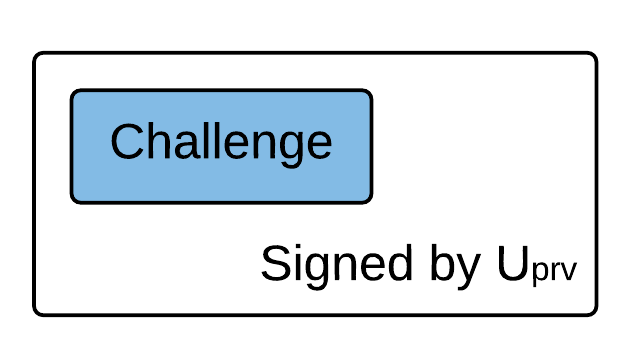
\includegraphics[width=0.65\textwidth]{images/challenge.png}
\end{figure}

\begin{figure}[h!]
  \caption{Smart card policy challenge response.}
  \label{fig:NH}
  \centering
    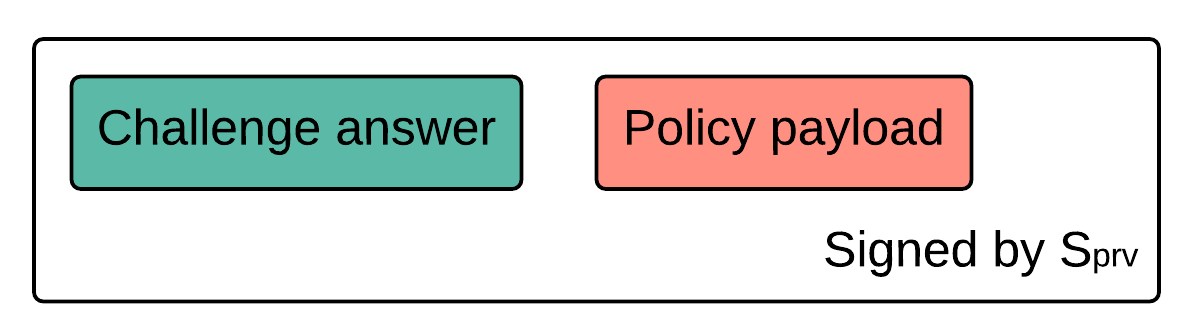
\includegraphics[width=0.75\textwidth]{images/challenge_response.png}
\end{figure}

\newpage

\paragraph{Challenge transaction}\mbox{}\\

U - Users smart card \\
M - Mobile device \\
S - Server, representation of authority \\
OH - Original hash \\
NH - New hash \\
\{Entity\}\textsubscript{prv} - Private key of an entity (U, M, S)\\

First we assume the binding of card and phone from section \ref{sec:bindingcardandphone} was successful. Secondly we assume that the server and smart card has a shared secret: a securely generated 256-bit AES key.

\begin{enumerate}
    \item U generates a challenge which is a long random hash (OH).
    \item U signs OH with U\textsubscript{prv}.
    \item U sends the signed OH package to S via the mobile device.
    \item S computes new hash (NH) using the AES key S and U agreed upon.
    \item S signs NH and the policy update.
    \item S sends the signed NH package (with policy update) to U via the mobile device.
    \item U computes the new hash and compares it to the NH it received.
    \item U applies policy updates.
\end{enumerate}

\begin{figure}[h!]
  \caption{Smart card policy challenge.}
  \label{fig:SQD_policy}
  \centering
    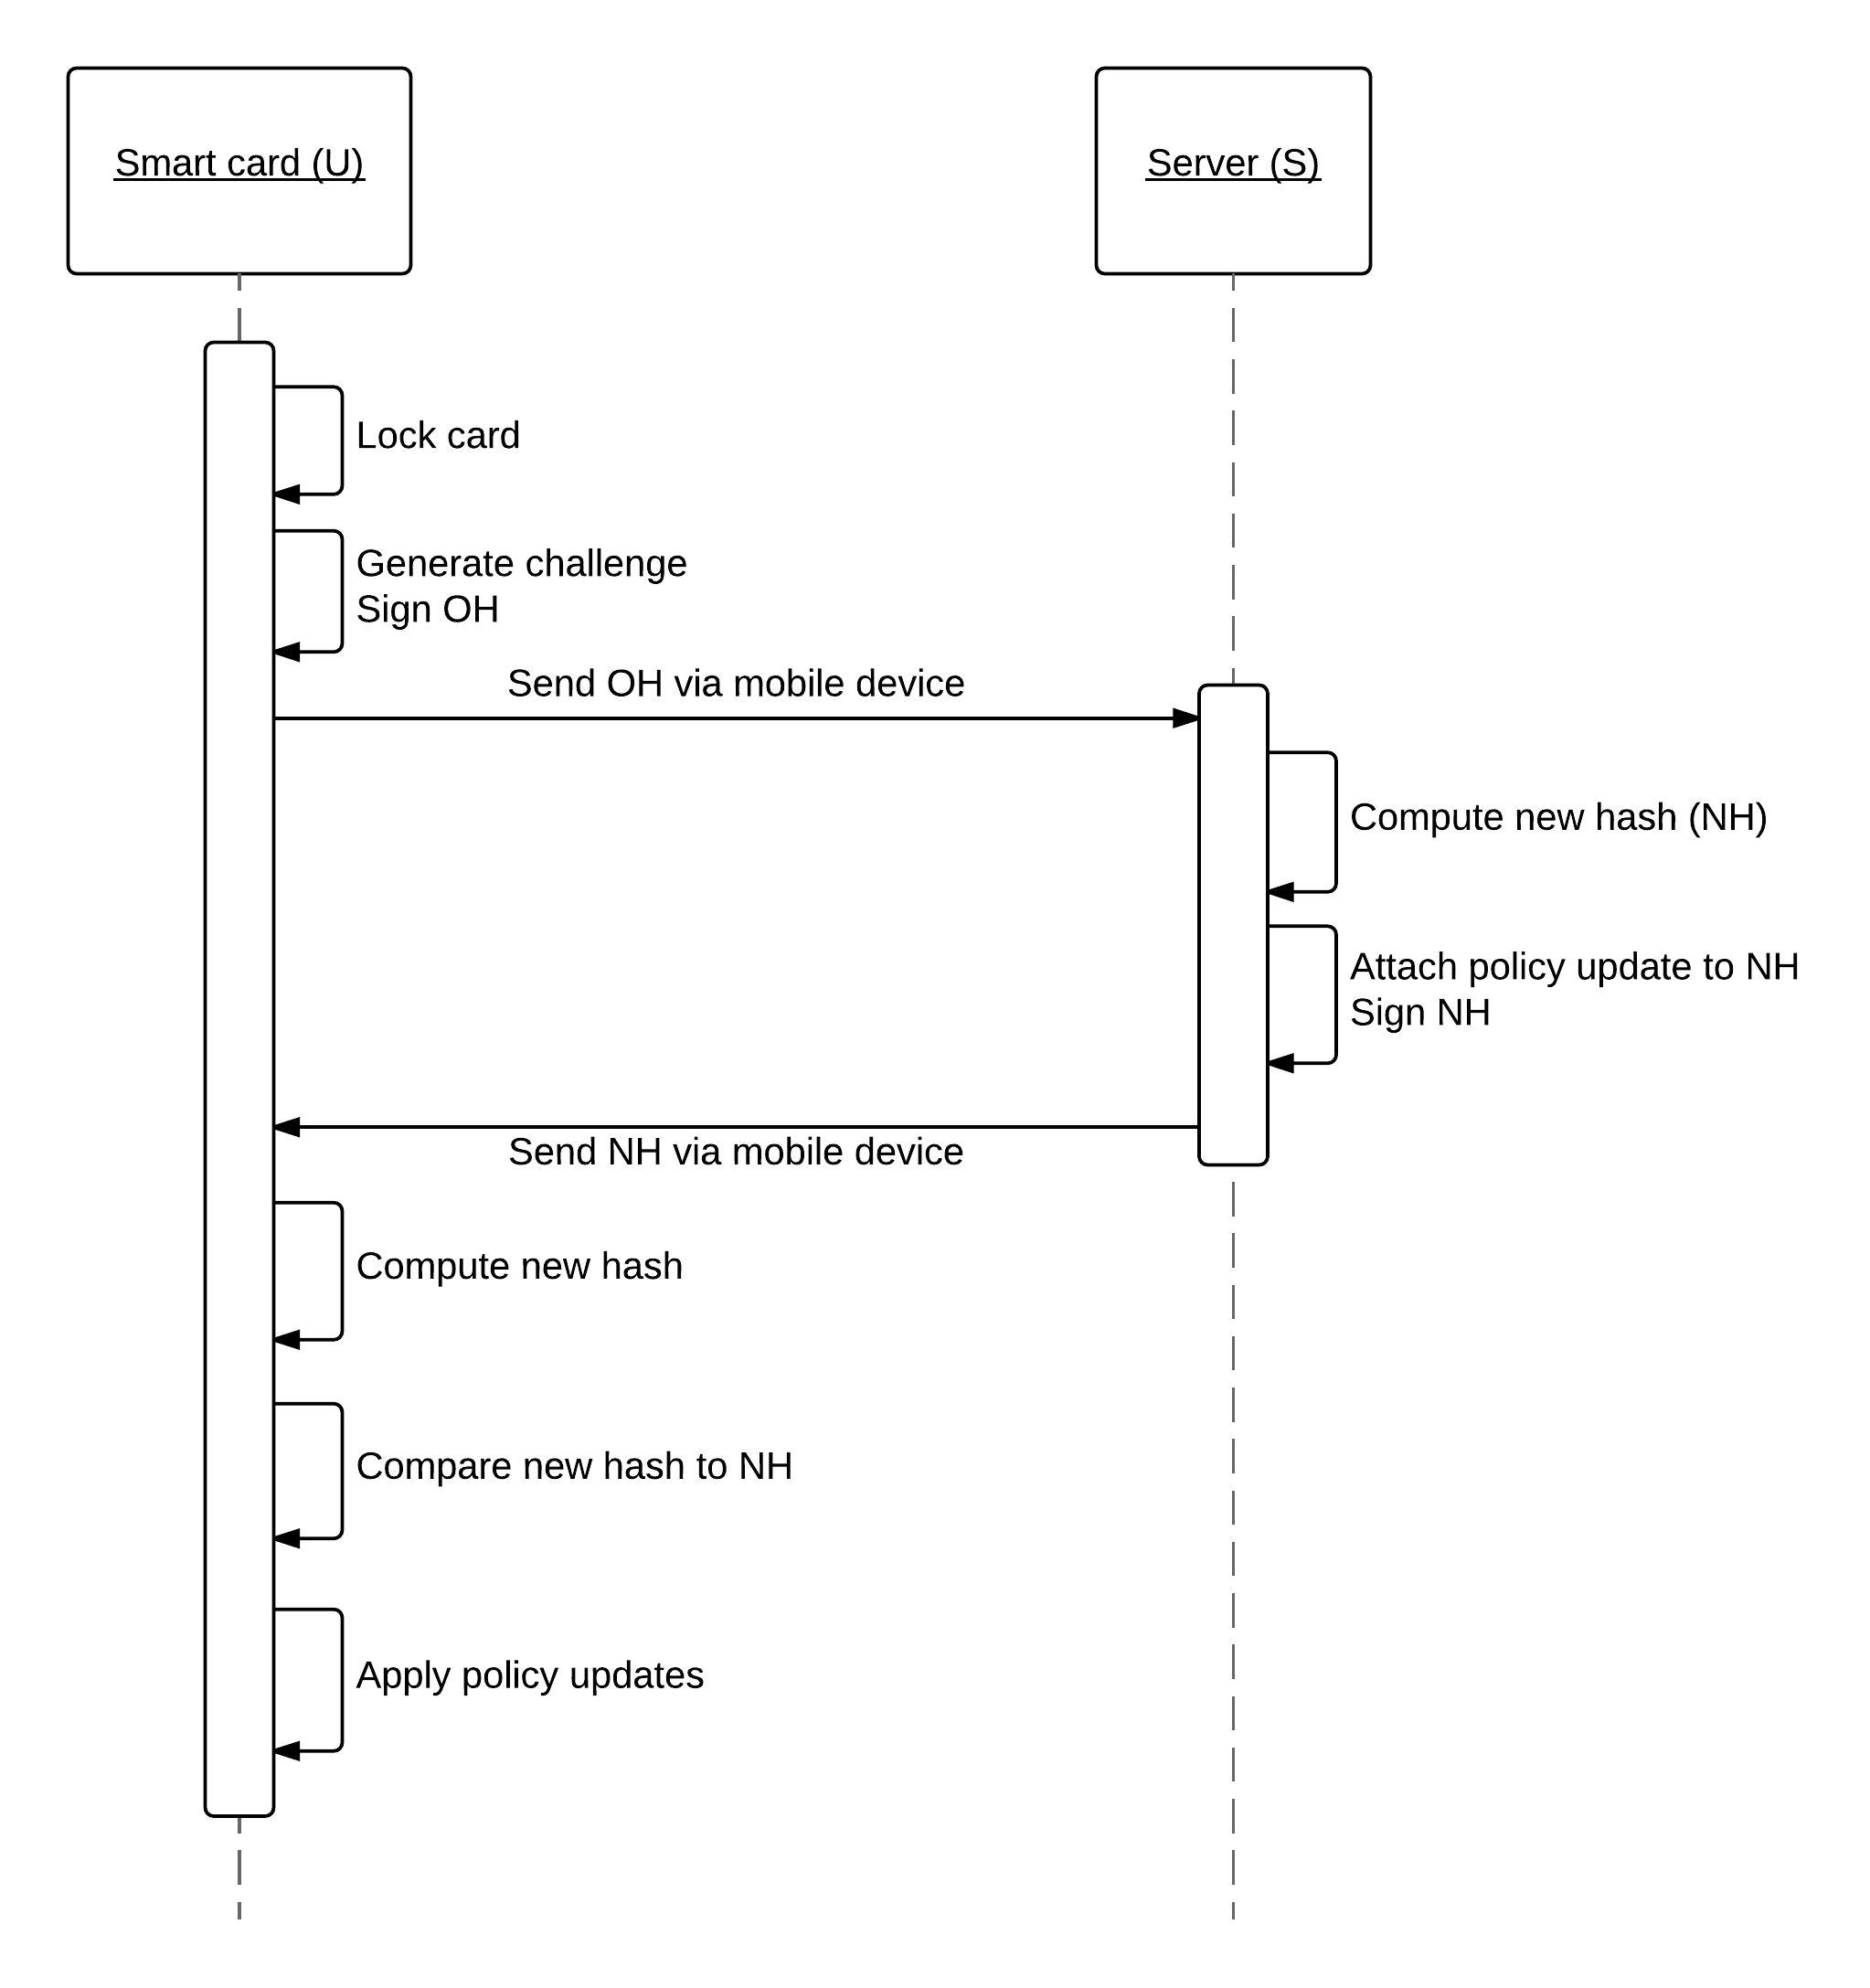
\includegraphics[width=0.95\textwidth]{images/SQD_Policy_Exchange.png}
\end{figure}

\newpage
%The "challenge" consists of a long random hash which is then signed by the smart card and sent to the server via the mobile device (see figure). The server computes the new hash using the AES key the smart card and server agreed upon. The new hash and any policy update is signed by the server and sent to the smart card.

\paragraph{Policy format}\mbox{}\\
When designing the format of the policy package there are two things to keep in mind. It should be human-readable for easy modification and not deviate too far from a machine-readable format as the smart card will need to interpret it. Another requirement to take into consideration is that data being sent to the smart card, must be converted to hex.

We can utilize JSON to make human-readable policies and as an added bonus JSON is readable for most programming languages. Listing \ref{lst:jsonPolicies} shows how this can be structured.
\begin{lstlisting}[language=json,firstnumber=1,caption=Human-readable policies in JSON., label=lst:jsonPolicies,]
{
  "policies": [
    {
      "id": "19",
      "description": "PIN attempts",
      "enabled": "true",
      "attempts": "3"
    },
    {
      "id": "21",
      "description": "Keylength (AES)",
      "enabled": "true",
      "keyLength": "256"
    }
  ]
}
\end{lstlisting}

Recall section \ref{sec:communicationstandard} where we described how a Command APDU must be structured. In the header we can use INS as a flag for ``policy update instruction'', for instance \texttt{09}. Next we have to look at what we technically want to achieve:
\begin{enumerate}
    \item Set boolean variable to true, depending on policy ID and ``enabled'' flag.
    \item Set other variable values.
\end{enumerate}
In the body we will use the payload data field to send information on the policy updates. The incoming data will be in byte format. Mapping bytes to variables could normally be solved using \texttt{HashMap} and map entries with \texttt{<byte, Object>}; the first parameter is the incoming byte command and second parameter being the variable we want to manipulate. \texttt{HashMap} is not a part of the Java Card API and we need to do our own hardcoded manual mapping. The result is a rigid structure for policies.

The individual policies data structure needs to be carefully crafted and specialized, but we should also focus on making it as dynamic as possible. This is best described using an example. To demonstrate how it can be done, we will use listing \ref{lst:jsonPolicies} as example data. The resulting APDU is figure \ref{fig:policyAPDU} and it clearly shows that we have to hardcode how many fields a policy will need.

\begin{figure}[h!]
  \caption{Example policy APDU with two policies}
  \label{fig:policyAPDU}
  \centering
    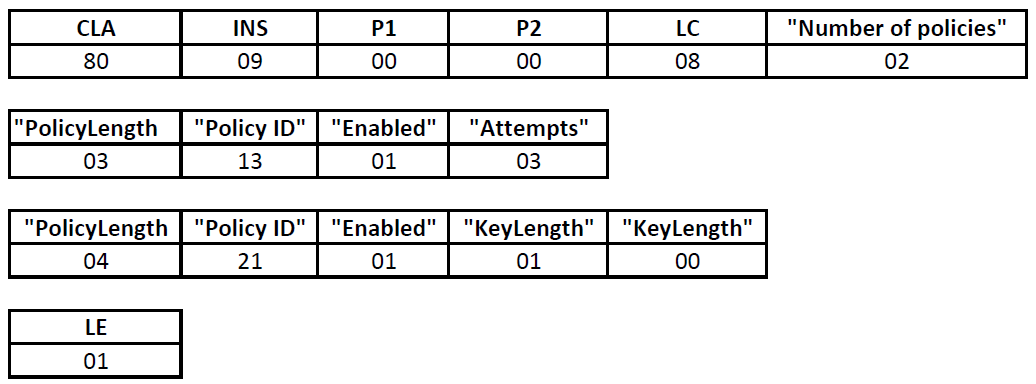
\includegraphics[width=0.95\textwidth]{images/policyAPDU.png}
\end{figure}

When designing the smart card code for interpreting the policy APDU we need a registry of some sort for keeping track of how much of the payload each policy uses. Listing \ref{lst:apduPolicy} uses figure \ref{fig:policyAPDU} as incoming APDU.

\begin{lstlisting}[caption=Pseudo code for interpreting policy APDU with Java Card., label=lst:apduPolicy,escapechar=å]
public class cardApplication extends Applet implements å\allowbreak åExtendedLength{
    ...

    //Policies
    final short offset = 5;
    short counter;

    //Policy 13
    boolean enabled13;
    short attempts;

    //Policy 21
    boolean enabled21;
    short keyLength;

    public void process(APDU apdu) {
    	...
        byte[] buff = apdu.getBuffer();

    	switch(buff[ISO7816.OFFSET_INS]){
            case 0x09:
                counter = 6;
                for(short i = 0; i < buff[offset]; i++){
                    if(buff[counter+1] == 13){
                        enabled13 = (buff[counter + 2] != 0);
                        attempts = buff[counter + 3];
                    }
                    else if(buff[counter+1] == 21){
                        enabled21 = (buff[counter + 2] != 0);
                        keyLength =
                            (short)((buff[counter+3]<<8)
                             | (buff[counter+4]))
                    }
                    counter += (1 + buff[counter]);

                }
                break;


            ...

    	}
    	Send(apdu);
    }

    private void send(APDU apdu) {
    	//Package outgoing buffer
    	//Send response APDU
    }
}
\end{lstlisting}

\subsection{Solution evaluation}
Section \ref{sec:policySolution} described how a smart card can enforce policies and how to manage policies. The solution is complex, intricate, requires a lot of overhead and is very rigid. Despite these drawbacks, using a smart card for policy enforcement could be well worth it. If an organization need a system where they are in full control and that is tamper proof, a smart card solution is viable option.

\subsection{Potential attack vectors}
\paragraph{Known-plaintext attack}\mbox{}\\
The challenge we use is simply two parties creating the same ciphertext from a hash and then comparing them. We then use digital signing to ensure that the challenge-response cannot be intercepted and spoofed. Since we do not encrypt the challenge-response in any way we have to vary of ``known-plaintext attacks'' \cite[~Ch. 2.3.2]{cryptoMath}. To protect against this type of attack the smart card and server must use keys that are long and algorithms that cannot be brute-forced. The final solution should use at least 256-bit long AES keys and as an added measure rotate keys.






%end
